% Oles Hodych March 2009

\documentclass[k]{vakthesis}
% Існують кілька опцій, які необхідно вказувати як факультативний
% аргумент команди \documentclass. Для магістерської роботи m, курсової роботи k, дипломної роботи d.
% Наприклад, для курсової роботи необхідно написати
% \documentclass[k]{vakthesis}

% Налагодження кодування шрифта, кодування вхідного файла
% та вибір необхідних мов
\usepackage[T2A]{fontenc}
\usepackage[english,russian,ukrainian]{babel}

\usepackage{graphicx}
\usepackage{subfigure}
\usepackage{alltt}
\usepackage{moreverb}
\usepackage{setspace}
\usepackage{algorithmic}
\usepackage{algorithm}
\usepackage{multirow}
\usepackage{bigstrut}
\usepackage{makecell}
\usepackage[table]{xcolor}
\usepackage{tabularx}
\usepackage{wrapfig}% використаний замість пакету floatflt, який був вилучений із texlive що постачається із ubuntu 10.04.
\usepackage{url}
\usepackage{array}
\usepackage{booktabs}
% Підключення необхідних пакетів. Наприклад,
% Пакети AMS для підтримки математики, теорем, спеціальних шрифтів
\usepackage[intlimits]{amsmath}
\allowdisplaybreaks
\usepackage{amsthm}
\usepackage{amssymb}
% Налагодження нумерованих списків
%\usepackage{enumerate}
% Гіпертекстові документи
%\usepackage{hyperref}
% або лише спеціальне форматування URL
%\usepackage{url}
% У списку літератури зворотні вказівки на посилання
%\usepackage{backref}
% Сортування посилань
%\usepackage[noadjust]{cite}
% Останні два пакети несумісні між собою. Крім того, конфліктують з цим класом!

% Налагодження параметрів сторінки (зокрема берегів).
% Наприклад, за допомогою пакета geometry
\usepackage{geometry}
\geometry{hmargin={30mm,15mm},vmargin={26mm,26mm}}

% TikZ
\usepackage[version=0.96]{pgf}
\usepackage{tikz}
\usetikzlibrary{arrows,shapes,shapes.arrows,shapes.misc,snakes,automata,backgrounds,petri,patterns,positioning,scopes,chains,matrix,decorations.pathmorphing,shadows}

% Означення теорем (теоремоподібних структур)
% Класичний варіант: для кожної теореми свій лічильник,
% тобто теорема 1.1, лема 1.1, теорема 1.2
\theoremstyle{plain}
\newtheorem{theorem}{Теорема}[chapter]
\newtheorem{lemma}{Лема}[chapter]
\newtheorem{corollary}{Наслідок}[chapter]
\theoremstyle{definition}
\newtheorem{definition}{Означення}[chapter]
\newtheorem{example}{Приклад}[chapter]
\theoremstyle{remark}
\newtheorem{remark}{Зауваження}[chapter]
\theoremstyle{statement}
\newtheorem{statement}{Твердження}[chapter]
\usepackage{listings}

% Цікавий варіант: всі теореми нумеруються одним лічильником,
% тобто теорема 1.1, лема 1.2, теорема 1.3
%\theoremstyle{plain}
%\newtheorem{theorem}{Теорема}[chapter]
%\newtheorem{lemma}[theorem]{Лема}
%\newtheorem{corollary}[theorem]{Наслідок}
%\theoremstyle{definition}
%\newtheorem{definition}[theorem]{Означення}
%\newtheorem{example}[theorem]{Приклад}
%\theoremstyle{remark}
%\newtheorem{remark}[theorem]{Зауваження}

% Якщо потрібно працювати лише з деякими розділами
%\includeonly{xampl-ch1,xampl-bib}

% Інформація про використані пакети тощо.
% Може знадобитися для відлагодження класу документа
%\listfiles

% custom commands
\def\argmin{\mathop{\rm arg\,min}} %define \argmin command

\begin{document}

%%%%%%%%%%%%%%%%%%%%%%%%%%%%%%%%%%%%%%%%%%%%%%%%%%%%%%%%%%%%%%%%%%%%%%%%
%%%%%%%%%%%%%%%%%%%%%%%%% Tkz styles %%%%%%%%%%%%%%%%%%%%%%%%%%%%%%%%%%%
%%%%%%%%%%%%%%%%%%%%%%%%%%%%%%%%%%%%%%%%%%%%%%%%%%%%%%%%%%%%%%%%%%%%%%%%
\tikzset{
  terminal/.style={
    % The shape:
    rounded rectangle,
    minimum size=6mm,
    % The border:
    very thick,
    draw=green!50!black!50,         % 50% red and 50% black,
                                  % and that mixed with 50% white
    % The filling:
    top color=white,              % a shading that is white at the top...
    bottom color=green!50!black!20, % and something else at the bottom
    % Font
    font=\itshape,text centered
  },
  process/.style={
    % The shape:
    rectangle,
    % The size:
    minimum size=6mm,
    % The rest
    very thick,draw=black!50,
    top color=white,bottom color=black!20,
    font=\ttfamily,text centered
  },
  decision/.style={
    % The shape:
    diamond, 
    minimum size=6mm,    
    % The rest
    very thick,draw=black!50,
    top color=white,bottom color=black!20,
    font=\ttfamily,text centered
  },
  data/.style={
    % The shape:
    trapezium,
    trapezium left angle=70, 
    trapezium right angle=110,    
    minimum size=6mm,    
    % The rest
    very thick,draw=black!50,
    top color=white,bottom color=black!20,
    font=\ttfamily,text centered
  },
  line/.style={draw, very thick, color=black!50,rounded corners},
  help-lines/.style={draw, very thin, color=black!50},
  arrow/.style={draw, very thick, color=black!50, -latex',rounded corners},
  helper-arrow/.style={draw, very thin, color=black, -latex'},
  dashed-line/.style={draw, dashed, color=black},
  point/.style={coordinate}
}
%%%%%%%%%%%%%%%%%%%%%%%%%%%%%%%%%%%%%%%%%%%%%%%%%%%%%%%%%%%%%%%%%%%%%%%%
%%%%%%%%%%%%%%%%%%%%%%%%%%%%%%%%%%%%%%%%%%%%%%%%%%%%%%%%%%%%%%%%%%%%%%%%
%%%%%%%%%%%%%%%%%%%%%%%%%%%%%%%%%%%%%%%%%%%%%%%%%%%%%%%%%%%%%%%%%%%%%%%%


\floatname{algorithm}{Алгоритм} 
% Назва дисертації, курсової, магістерської
\title{Це стаб для оформлення дисертації, курсової, магістерської}
% Прізвище, ім'я, по батькові здобувача
\author{Прізвище Автора Роботи}
% Прізвище, ім'я, по батькові наукового керівника/консультанта
\supervisor{Прізвище Керівника Роботи}
% Науковий ступінь, вчене звання наукового керівника/консультанта
           {кандидат фізико-математичних наук, доцент}
% Спеціальність
%\speciality{01.05.03}[технічних наук]
% Варіант із вказуванням факультативних аргументів
\speciality{01.05.03}
% Індекс за УДК
\udc{004.853+004.855.5}
% Установа, де виконана робота, і місто
\institution{НУ ``Львівська політехніка''}{Львів}
% Рік, коли написана (подана до захисту?) дисертація
\date{2012}

% Тут буде титульна сторінка
\maketitle

% Зміст
\setcounter{tocdepth}{2} % контролює рівень заголовків, які повинні відображатись у змісті
\tableofcontents
\nocite{*}
%\listoftables 
%\listoffigures

\lstset{basicstyle=\footnotesize, language=Java,morekeywords={val,def,object}}

% Розділи дисертації в окремих файлах
%% ����� �� ����������
%% ������� �������������� ������
\chapter*{�����}

\paragraph{������������ ����}

�� ��������� �� ���������� ������������� ������� � ����� ������� �������� ������ ��'��� �����, �� ����������� � ������ �� ����� �����, ����������� �������� �������. �������� �����������, �� �������� �� ���� ������, ���������� ������ ������ ��������� � ��� ����������. 

\paragraph{���� � �������� ����������}
����� ���������� � ��������\ldots. ��� ���������� ���� ���� ���� ������������� �� ������� ��� ������� ��������:

\begin{itemize}
 \item �������� ����������� ����� �� �������� ������������\ldots;
 \item ��������� ������ �� ���������, �� ������������� ������\ldots; 
 \item �������� �������������\ldots;
 \item ��������� ����� ������������ �� �������� ��������\ldots;
 \item ��������� ����������� �� ��������� ������������\ldots
\end{itemize}

\subparagraph{��'��� ����������}
���������� ������ ��������������� ������� ����� �� ����� ���� �������� � ��'����� ����������.

\emph{\textbf{��'����� ����������}} � �������\ldots

\emph{\textbf{��������� ����������}} � ������\ldots 

\paragraph{��������� ����������}

������ ���������� � ������, ����� ������, ��������. ����� ������� 50~������� ������, ������ ������������ ������ ������ 20~������������).%                                                      Вступ
%% problem-overview.tex  
% цей розділ присвячений огляду стану проблеми
\chapter{Огляд стану проблеми та основні поняття}\label{ch:01}

Моделювання даних завжди було невід'ємною частиною побудови інформаційних систем. Уважається, що інженери Young та Kent \cite{YoKe1958} першими висловили необхідність у чіткому та абстрактному способі специфікації інформаційних та часових характеристик проблем опрацювання даних. Значним поступом у розвитку моделювання даних, та інформаційних систем узагалі, стала праця дослідницької групи CODASYL (англ. COnference on DAta SYstems Language) \cite{CODASYL1962}. Важливим результатом CODASYL є розробка інформаційної алгебри \cite{Kal1983}, відповідно до якої, властивості об'єктів розглядають як відображення $p_k:E\rightarrow V_k$, де $E$ -- множина об'єктів предметної області, а $V_k$ -- множина значень властивості $p_k$. Об'єкти подаються у моделі впорядкованими значеннями його властивостей $p_1,\cdots,p_m$, які є координатами універсального інформаційного простору $V=V_1\times V_2\times\cdots\times V_m$. Ідеї інформаційної алгебри були, зокрема, використані в реляційній та семантичній моделях даних \cite{Oli2009}\ldots

\subsection{Підрозділ}

\subsection{Ще одни підрозділ}

\section{Висновки до розділу~\ref{ch:01}}%                                Розділ 1
%% the-core.tex  
% ��� ����� ����������� ���������� ������ ����, ������ �� ���������
\chapter{������ �� ��������\ldots}\label{ch:02}

���� � ������ ���������� ����, ����������� �������� ���������������, �������� ����������~\cite{Ros1963}, � ���� ��������� ������� ���, ������������� ��� ������������ ������� ������� ��������� �����. ������������� ������ �� ���� ����������� ����������, ��� ������� ������� ���  ��������� ���������~\cite{ShlHlav2004}. � ������ ���������� ����������� ������ �� ����� ������� ��������������� ������������ �������� ������ �.�. ���������, ���� ���� ������ ��������� ������ ��� ���������� �����������~\cite{Iva1982}. ������������ ����� ��������� ������ ����������� ��������~\cite{MaIv1994}.

\section{������ �������}\label{ch:0201}

�� ��������� � ���������㳿 �����, �� ���� ������� ���� ��������� ����� ������������ � ���������� �� ����� ���� �����~\cite{Koh2001}. ���� ������ ���������� ��������� ����� �������� �� ��, �� �������-������� ���������� �� ��� ��������� ����� � ���� ������ ������������ �������, � ����� ���� ���� �������� �������� ����� (���������, �����). ����� �������� ������� ���� ������ ��������, ������� ����������� �������� �������� �� ������ ���� �������� � ���������� ������������� �����. ����� ��'���� �� �������� �������������� ��������� ����� ������� ������������ ���� �������� �� ������ ����������� ������� ��������� �����~\cite{RMS1992}. ���� ����� �������� ����� ��������� \emph{������������ ��������}, � �� �������� -- \emph{���������}.

\subsection{������ ������� ������� ��������}

\begin{table}
   \centering
   \caption{������� ������}
   \label{tbl:medical-data-fragment}
   \def~{\phantom{0}}
   \def\ExSp#1{\noalign{\vskip #1}}
   \def\Hline{\noalign{\hrule height 2\arrayrulewidth}}
   \begin{tabular}{cccccccccccccccc}
     \ExSp{0.2ex} \Hline \ExSp{1ex}
     \rotatebox{45}{\tiny AGE} & \rotatebox{45}{\tiny G} & \rotatebox{45}{\tiny PIK} & \rotatebox{45}{\tiny KHK\_AKMK} & \rotatebox{45}{\tiny KV} & \rotatebox{45}{\tiny SK} & \rotatebox{45}{\tiny UA} & \rotatebox{45}{\tiny AA} & \rotatebox{45}{\tiny BE} & \rotatebox{45}{\tiny OH} & \rotatebox{45}{\tiny REW} & \rotatebox{45}{\tiny R\_AK} & \rotatebox{45}{\tiny R\_MK} & \rotatebox{45}{\tiny R\_AKMK} & \rotatebox{45}{\tiny GH} & \rotatebox{45}{\tiny KHKS}\\
     \ExSp{0.2ex} \hline\ExSp{1ex}
     0 & 1 & 0 & 0 & 0 & 0 & 0 & 0 & 0 & 0 & 0 & 0 & 0 & 0 & 1 & \cellcolor[gray]{0.9}1\\
     1 & 1 & 1 & 0 & 0 & 0 & 0 & 0 & 0 & 0 & 1 & 0 & 0 & 1 & 0 & \cellcolor[gray]{0.9}0\\
     1 & 0 & 1 & 1 & 0 & 0 & 0 & 0 & 0 & 0 & 0 & 0 & 0 & 0 & 1 & \cellcolor[gray]{0.9}1\\
     1 & 1 & 1 & 1 & 0 & 0 & 0 & 0 & 0 & 0 & 0 & 0 & 0 & 0 & 1 & \cellcolor[gray]{0.9}1\\
     \ExSp{1ex} \hline
   \end{tabular}
\end{table}

\begin{table}
  \centering
  \caption{������� �� ������ �������}
  \label{tbl:medical-data-stats}        
  \def~{\phantom{0}}
  \def\exsp#1{\noalign{\vskip #1}}
  \def\hline{\noalign{\hrule height 2\arrayrulewidth}}
  \begin{tabular}{ccccc}
  \exsp{0.2ex} \hline \exsp{1ex}
  \rotatebox{45}{\small�-��� ������} & \rotatebox{45}{\small³������ ������} & \rotatebox{45}{\small�-��� ��������} & \rotatebox{45}{\small³������ ��������} & \rotatebox{45}{\small�������� �-���}\\
  \exsp{0.2ex} \hline\exsp{1ex}
  756 & 21.6\% & 2744 & 78.4\% & 3500\\
  \exsp{1ex} \hline
  \end{tabular}
\end{table}

\subsection{������ ������� ������� ��������}

\begin{algorithm}[!htb]
\caption{������� ��������� ����� ����� ���������.}\label{alg:classifier}
\begin{enumerate}
\item[ ]\emph{������������.} ����������� ���� ������ $(a_i,b_i)$ ��� ������� �������� $m_i\in M$, �� ���������� ������� ��������� �������� �� ������ �� �������� ��������. ���������� $a_i\leftarrow 0$, $b_i\leftarrow 0$, $i=\overline{1,|M|}$. �������� ������� ������� �����, ��� ��� ����������������� ��������� ������������, ��� ��������� $T$. ������� ������� ��������-���������� $K\leftarrow\varnothing$.
\item[1.] �������� ������� ������ $x\in T$ � �������� ����, ���������� $T\leftarrow T\setminus\{x\}$.
\item[2.] ��� ������� $x$ ��������� ��������� $m(x)$ �������� �� ������������~(\ref{eq:winner}); ��������� $K\leftarrow K\cup\{m(x)\}$.
\item[3.] ���� ������� $x$ ������� ������ ��������� ����� � �������� 1 (���� ��������), �� ��������� $a_{m(x)}\leftarrow a_{m(x)} + 1$, ������ -- $b_{m(x)}\leftarrow b_{m(x)} + 1$.
\item[4.] ���� $T\neq \varnothing$, �� ����������� �� ���� 1.
\item[5.] ��������� ��������� ������� �������� $m\in K$:\\$s_k=\dfrac{\xi_k}{a_k + b_k}*100$, $k\in I(K)$, �� $I(K)$ -- ������� ������� ��������-����������, $\xi_k=\left\{\begin{array}{r@{,\quad}l}a_k & a_k\geq b_k \\ b_k & a_k < b_k\end{array}\right.$
\item[6.] ���������� �������� ��������� ������������: \begin{eqnarray*}S=\dfrac{1}{|K|}\sum_{k=I(K)}s_k,\end{eqnarray*} �� $|K|$ -- ������� ��������-���������� ��� ������� ������� $T$.
\end{enumerate}
\end{algorithm}

\section{�������� �� ������~\ref{ch:02}}
� ����� ����� �������� ���������� ����������\ldots%                                                Розділ 2
%% software-and-experiments.tex  
% цей розділ висвітлює програмне рішенні та результати експериментів дослідження
\chapter{Об'єктно-орієнтоване програмне\ldots}\label{ch:03}

  Одним із найгнучкіших підходів до практичної реалізації нейромережевих технологій є створення програмного рішення. Цей підхід забезпечує можливість легкої модифікації реалізації порівняно з апаратними рішеннями\ldots 
  
\section{Структура та характеристики}
  
  При розробці програмного забезпечення було поставлено за мету використання виключно відкритого та вільного програмного забезпечення\ldots
  
  На рис.~\ref{fig:neurosimulator-modules} зображена компонентна діаграма розробленого програмного забезпечення із виділеними допоміжними модулями ресурсної взаємодії через Інтернет~\cite{Fie2000} та об'єктно-орієнтованої взаємодії з системами керування реляційними базами даних~\cite{ChGa2006}. 
  
  \begin{figure}[!htb]
    \centering
    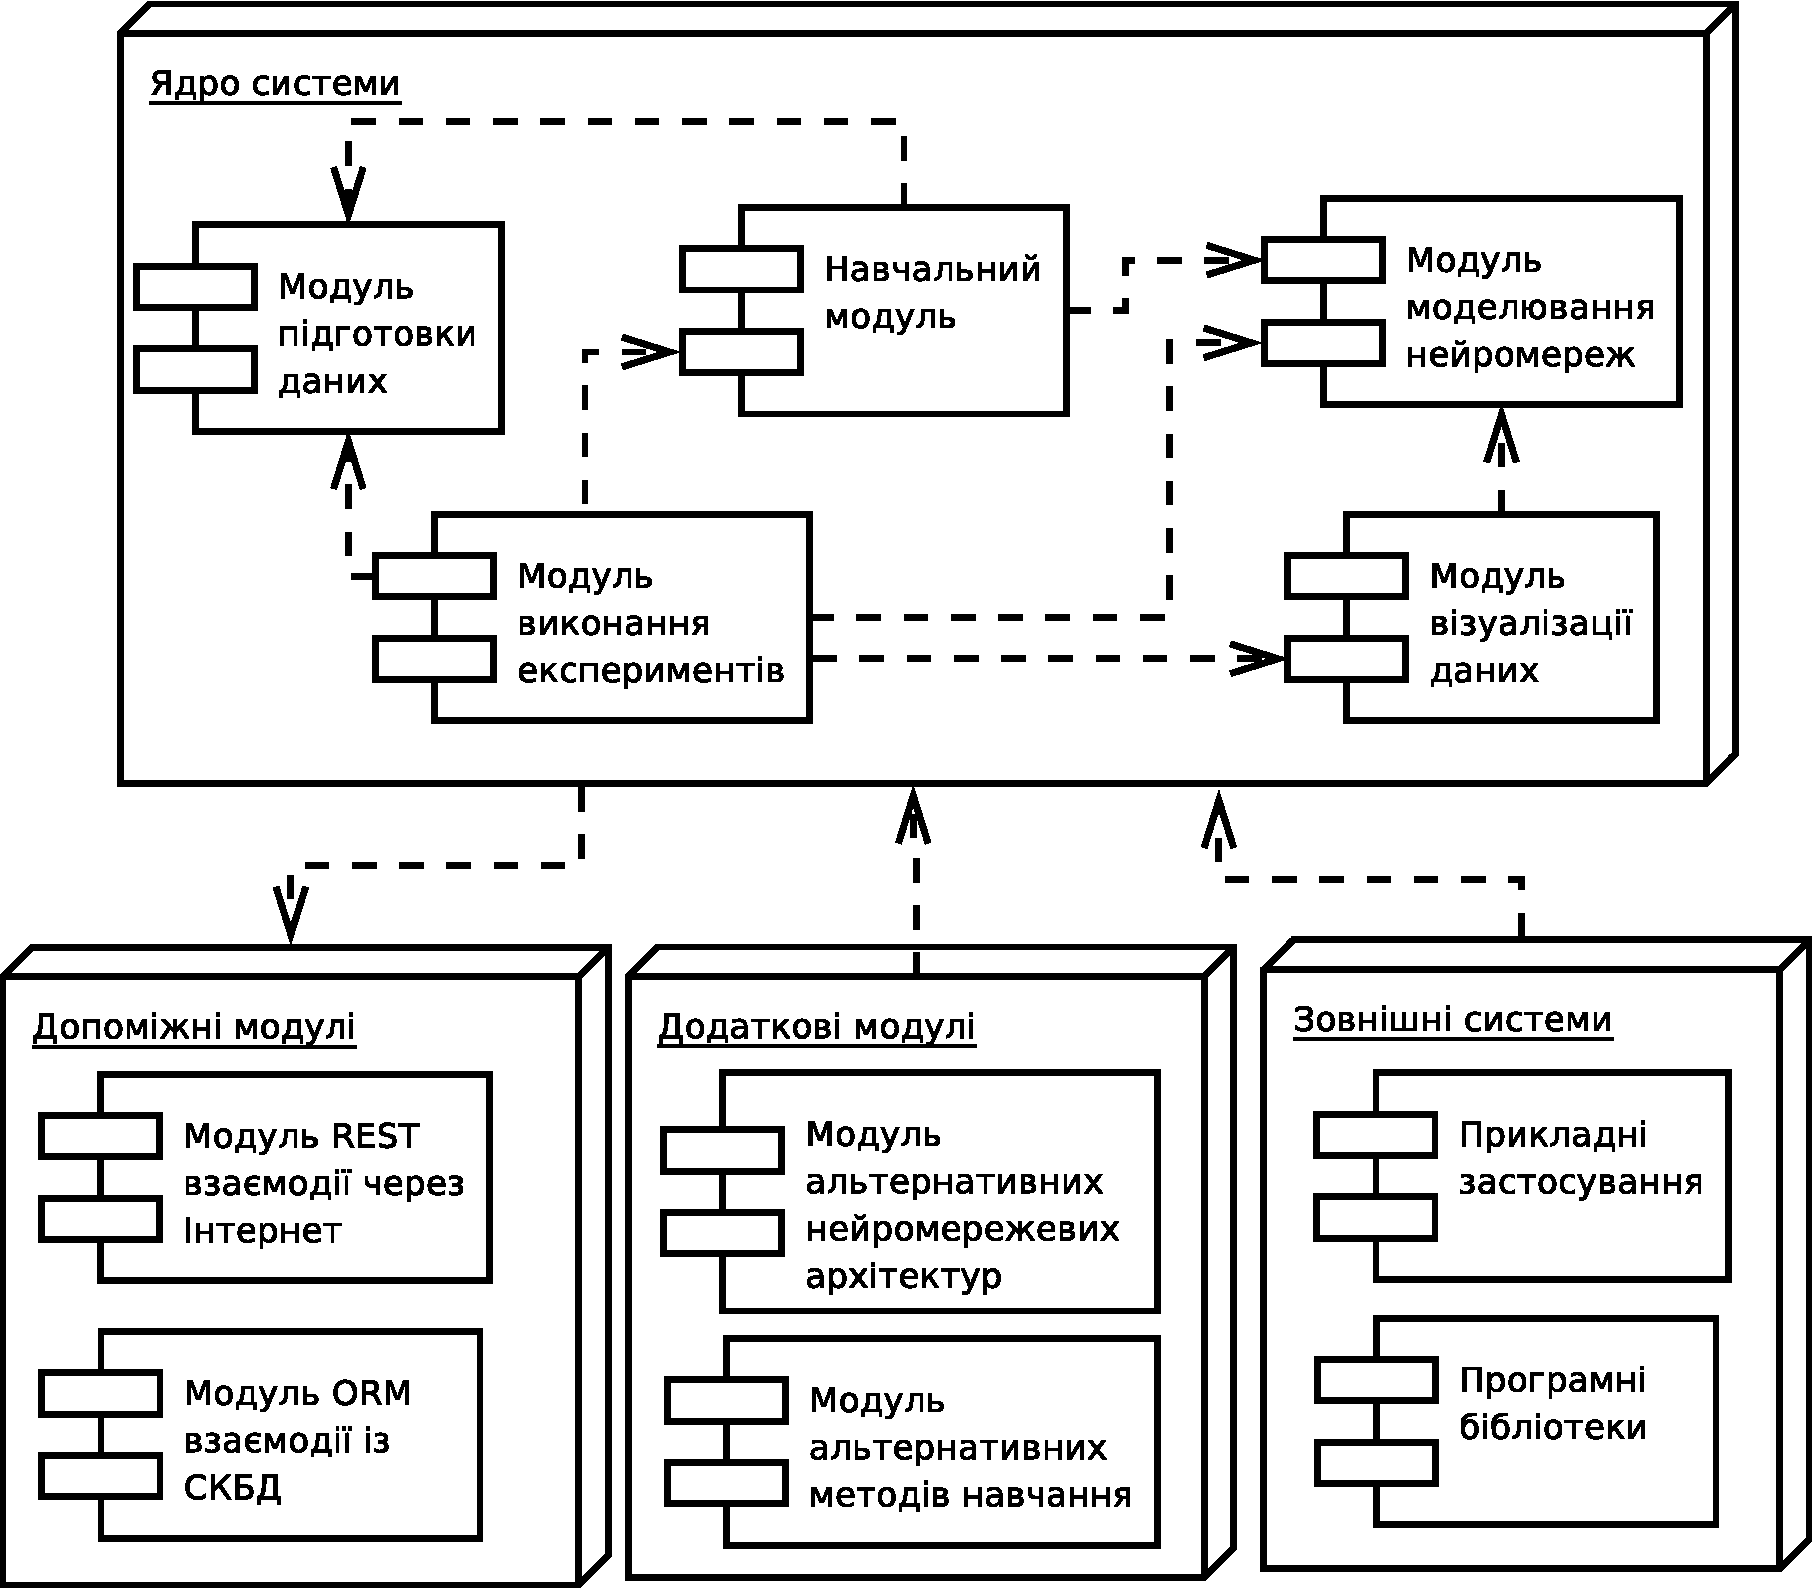
\includegraphics[scale=0.5]{chapters/03-software-and-experiments/images/01-neurosimulator-component-diagram.pdf}%
    \caption{Компонентна діаграма розробленого програмного забезпечення.}\label{fig:neurosimulator-modules}
  \end{figure}
  
  
\section{Обговорення коду}

\begin{lstlisting}
def filter(p: Tweet => Boolean): TweetSet
def filter0(p: Tweet => Boolean, 
            accu: TweetSet): TweetSet
\end{lstlisting}


\section{Висновки до розділу~\ref{ch:03}}%                Розділ 3
%% conclusion.tex  
% тут робимо остаточні висновки
\chapter*{Висновки}\label{ch:04}

У курсовій роботі вирішено актуальну науково-прикладу задачу розвитку\ldots

При цьому було отримано такі наукові результати.
\begin{enumerate}
 \item що, яким чином і який ефект було досягнуто;
 \item що, яким чином і який ефект було досягнуто;
 \item що, яким чином і який ефект було досягнуто;
 \item що, яким чином і який ефект було досягнуто.
\end{enumerate}%                                            Висновки
%% ������� �����-�������� ��� ������/������ ���������
% ��� ���������� ��������� �� �������� �������������� gost780s
\bibliographystyle{gost780s}
\bibliography{chapters/05-bibliography/sources}
%                                        Список використаних джерел (+список публікацій автора)

\end{document}